%%%%%%%%%%%%%%%%%%%%%%%%%%%%%%%%%%%%%%%%%%%%%%%%%%%%%%%%%%%%%%%%%%%%%%%%%%%%%%%%%%%%%%%%%%%%%%%%%%%
%%%%%%%%%%%%%%%%%%%%%%%%%%%%%%%%%%%%%%%%%%%%%%%%%%%%%%%%%%%%%%%%%%%%%%%%%%%%%%%%%%%%%%%%%%%%%%%%%%%
%%%%%%%%%%%%%%%%%%%%%%%%%%%%%%%%%%%%%%%%%%%%%%%%%%%%%%%%%%%%%%%%%%%%%%%%%%%%%%%%%%%%%%%%%%%%%%%%%%%
%%%%%%%%%%%%%%%%%%%%%%%%%%%%%%%%%%%%%%%%%%%%%%%%%%%%%%%%%%%%%%%%%%%%%%%%%%%%%%%%%%%%%%%%%%%%%%%%%%%

\chapter*{Introducción}
\addcontentsline{toc}{chapter}{Introducción}

Gracias a los avances médicos del último siglo se ha incrementado la esperanza de vida y la calidad de vida. 
%
Desafortunadamente, también ha aumentado la presencia de enfermedades no-transmisibles asociadas con la edad. 
%
En México el sector de la población con más de 60 años de edad (considerados en alto riesgo para este tipo de enfermedades) contempló a 10 millones de personas en 2010, y en 2015 dicha cifra creció a 12 millones \cite{Censo10,Intercensal15}.
%
En este trabajo se destaca la demencia de entre las enfermedades asociadas con la edad.

La demencia consiste en el desarrollo de deficiencias cognoscitivas (especialmente en atención y memoria) suficientemente graves para interferir en las actividades del individuo.
%
Se considera que la demencia es irreversible, y no se han identificado curas definitivas \cite{PlanAlzheimer04}, debido a lo cual ha surgido un gran interés en definir y diagnosticar sus etapas tempranas.
%
El deterioro cognitivo leve (DCL), una etapa temprana de la demencia, se entiende como el desarrollo de deficiencias cognoscitivas \textit{objetivas} pero que no corresponden a daño físico del cerebro y no son lo suficientemente graves para calificarse como demencia.

Existen varios otros métodos alternativos para detectar --o definir-- el DCL; desde la autopercepción por parte del paciente, hasta análisis genéticos, químicos y de imagenología cerebral.
%
De entre estas técnicas se destaca a la polisomnografía (PSG), el registro conjunto de varias señales electrofisiológicas durante el sueño.
%
En particular, se considera una PSG compuesta por registros de electroencefalograma (EEG), electrooculograma (EOG) y electromiograma (EMG) para medir, respectivamente, actividad eléctrica cerebral, tono muscular y movimientos oculares.
%
El uso en particular de registros de PSG obedece principalmente a que (1) es una técnica relativamente barata y no invasiva, con relación al tipo de información que se obtiene, y (2) existe una cantidad moderadamente grande de marcadores para el DCL reportados usando la PSG.

Se ha encontrado, por ejemplo, correlaciones entre el DCL en adultos mayores con la \textit{presencia} de ciertos tipos de ondas cerebrales \cite{babiloni13,prichep94,prichep06}.
%
Sin embargo, otros estudios sugieren que el EEG durante el sueño es un mejor predictor del DCL [buscar y citar Baryet ??].

En el presente trabajo se busca desarrollar métodos para determinar el DCL en base a registros de PSG en adultos mayores, como complemento a los resultados de pruebas neuropsicológicas.
%
Se mantiene presente que el deterioro cognitivo (más allá del DCL) no puede reducirse exclusivamente a tales mediciones; las conclusiones obtenidas usando registros de señales electrofisiológicas deben ser contrastadas siempre con resultados de análisis complementarios.

%%%%%%%%%%%%%%%%%%%%%%%%%%%%%%%%%%%%%%%%%%%%%%%%%%%%%%%%%%%%%%%%%%%%%%%%%%%%%%%%%%%%%%%%%%%%%%%%%%%
%%%%%%%%%%%%%%%%%%%%%%%%%%%%%%%%%%%%%%%%%%%%%%%%%%%%%%%%%%%%%%%%%%%%%%%%%%%%%%%%%%%%%%%%%%%%%%%%%%%

\section*{Antecedentes}
\addcontentsline{toc}{section}{Antecedentes}

Se considera que la técnica de EEG fue inventada en la década de 1920 por el fisiólogo Hans Berger, quien descubrió que ésta es \textit{sensible} a cambios en la actividad mental como la concentración o el parpadeo de voluntario.
%
Desde entonces se estableció que hay una conexión innegable entre el funcionamiento de la mente y los fenómenos eléctricos en el cerebro.
%
Después de casi un siglo, se ha llegado a aceptar que dicha asociación es más bien complicada.

Los fenómenos eléctricos en el cerebro que dan origen al EEG son conocidos, cuando menos en su \textit{nivel de organización} más básico: las neuronas
%


Por un lado el EEG es en parte un fenómeno eléctrico, tradicionalmente se le describe en términos de ondas y frecuencias, en ocasiones como un sistema dinámico.
%
Paralelamente el EEG es un fenómeno biológico, de modo que se le atribuyen características estocásticas pero --de alguna forma-- organizadas.
%
En su libro \textit{``Cybernetics or Control and Communication in the Animal and the Machine"}, el matemático Norbert Wiener comenta la posibilidad de que la actividad cerebral tenga un poco de ambas características, lo cual no lo excusa de ser estudiado formalmente (es decir, sin vageudad) como un sistema \cite{wiener61} cap11.

En el presente trabajo se opta por interpretar (como sinónimo informal para \textit{`modelar'}) a los registros de EEG como procesos estocásticos cuyo espectro de potencias es relevante; naturalmente, ambos términos serán definidos con detalle en el texto.

La actividad eeeg representa unn paradigma de complejidad, que no es sinónimo de complicadion sino de actividad emergente.
como los estados de agregacion de la materia.
el todo es mas que la suma de las partes
[?? citar articulo dfa vs patrones locales]

la estacionariedad local y dahlhaus.

El enfoque de estacionariedad, desde la perspectiva del espectro, ha sido tomado por varios autores. Por ejemplo Kaplan, quien lo usa para definir fragmentos cuyo espectro de potencias es omogeneo. 

Los fragmentos son ni portantes porque

la clase cohen y diferentes espectros cambiantes en el teimpo

Se usa la prueba propuesta por Priestley y Subba Rao.
Por ejemplo Nason, quien usa la estacionairedad en vulcanologia para detectar cosas. La prueba de PSR es una de las mas rapidas porque es nlog(n)

tiempo, fft y computadoras: tiene sentido usar pruebas viejas y raras

ya se habian presentado resultados previos
En un estudio reciente, EEG de una noche polisomnografía de personas mayores con y sin deterioro cognitivo según las evaluaciones con el Neuropsi analizó el porcentaje de estacionariedad.  En sueño MOR el porcentaje fue menor que el del sueño NMOR y la vigilia, se obtuvo estacionariedad  como un índice para comparar NMOR versus sueño MOR en ambos grupos %\cite{Rosales-Lagarde17}.

En 2016 Vázquez-Tagle y colaboradores estudiaron el PDCL en adultos mayores del estado de Hidalgo con el método no lineal del Análisis de Fluctuaciones sin Tendencia (DFA, por sus siglas en inglés), encontrando efectivamente que los sujetos con PDCL presentan mayor ruido browniano en varias regiones en comparación con los pacientes sin PDCL\cite{VazquezTagle16}.

%%%%%%%%%%%%%%%%%%%%%%%%%%%%%%%%%%%%%%%%%%%%%%%%%%%%%%%%%%%%%%%%%%%%%%%%%%%%%%%%%%%%%%%%%%%%%%%%%%%
%%%%%%%%%%%%%%%%%%%%%%%%%%%%%%%%%%%%%%%%%%%%%%%%%%%%%%%%%%%%%%%%%%%%%%%%%%%%%%%%%%%%%%%%%%%%%%%%%%%

\section*{Pregunta de investigación y objetivos}
\addcontentsline{toc}{section}{Pregunta de investigación y objetivos}

Los registros de PSG en adultos mayores, modelados como procesos estocásticos, ¿pueden considerarse como débilmente estacionarios?
%
¿Dicha caracterización es afectada si el individuo presenta PDCL?

%%%%%%%%%%%%%%%%%%%%%%%%%%%%%%%%%%%%%%%%%%%%%%%%%%%%%%%%%%%%%%%%%%%%%%%%%%%%%%%%%%%%%%%%%%%%%%%%%%%

\subsection*{Objetivos}

Estudiar sobre pruebas estadísticas para detectar si una realización dada proviene de un proceso estocástico débilmente estacionario.
%
Usar tales pruebas sobre registros de PSG en adultos mayores con y sin PDCL.
%
Investigar si hay una relación entre la presencia de PDCL y la clasificación de los proceso estocásticos referidos como débilmente estacionarios.

\section*{Sobre la estructura del texto}
%\addcontentsline{toc}{section}{Sobre la estructura del texto}

Debido al enfoque aplicado del presente trabajo, esta porción del texto fue estructurada pensando en dos tipos de lectores: por un lado aquellos interesados principalmente en los objetos matemáticos involucrados y sus conexiones, y por otro lado quienes ven los mismos como herramienta y esperan entenderlos mejor.
%
Los temas fueron ordenados pensando en el primer tipo de lector.
%
Para el segundo tipo de lector, se ha preparado en la figura \ref{intro:estructura} un \textit{mapa} del texto, pero principalmente de los temas sobre matemáticas.

En el primer capítulo se abordan varios temas preliminares sin lujo de detalles, con la finalidad de presentar un texto autocontenido;
%
la finalidad del capítulo es definir formalmente los procesos estocásticos, espacios de Hilbert y estimadores.

En el segundo capítulo se definen los procesos estocásticos débilmente estacionarios, al conjunto de éstos se les da estructura de espacio de Hilbert, y finalmente se usa dicha estructura para definir el espectro de potencias como una generalización de la transformada de Fourier.
%
Una porción importante del capítulo trata sobre la estimación efectiva del espectro de potencias a partir de observaciones dadas de un proceso estocástico.

En el tercer capítulo se define el \textit{espectro evolutivo}, una generalización del espectro de potencias para una familia de procesos que no son débilmente estacionarios.
%
Al final se expone una aplicación aparente menor del espectro evolutivo, pero que es fundamental para el resto del presente trabajo: la prueba de Priestley Subba-Rao. 
%
Esta prueba verifica --como prueba de hipótesis-- si el espectro evolutivo de un proceso puede reducirse a un espectro de potencias; en otras palabras, si un proceso es débilmente estacionario.

En el cuarto capítulo se presentan conceptos de índole \textit{fisiológica}: psicología, psicometría, electrofisiología.
%
El objetivo del capítulo es describir el DCL y cómo se detecta, describir qué es el sueño y como se analiza (en este caso a partir de la polisomnografía), y mencionar la relación entre el sueño y el DCL.

En el capítulo quinto se describe cómo se utilizó la prueba de estacionariedad débil para estudiar los registros de polisomnografía.
%
En el capítulo sexto se discuten los resultados obtenidos, y se concluye que la técnica utilizada no es un marcador diagnóstico para el DCL; se reportan algunos hallazgos incidentales.

\begin{figure}
\centering
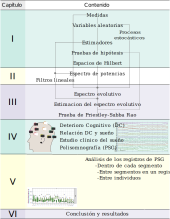
\includegraphics[width=.9\textwidth]{./estructura_texto_v2.pdf}
\caption[Estructura de la tesis]{Se ilustra gráficamente las \textit{dependencias} respecto a los tópicos de matemáticas, es decir, los temas que deben discutirse antes que otros. El resto del texto (incluyendo los tópicos de fisiología) son expuesto de forma más \textit{secuencial}, por lo que no se consideró necesario ilustrar sus dependencias.}
\label{intro:estructura}
\end{figure}

%%%%%%%%%%%%%%%%%%%%%%%%%%%%%%%%%%%%%%%%%%%%%%%%%%%%%%%%%%%%%%%%%%%%%%%%%%%%%%%%%%%%%%%%%%%%%%%%%%%
%%%%%%%%%%%%%%%%%%%%%%%%%%%%%%%%%%%%%%%%%%%%%%%%%%%%%%%%%%%%%%%%%%%%%%%%%%%%%%%%%%%%%%%%%%%%%%%%%%%
%%%%%%%%%%%%%%%%%%%%%%%%%%%%%%%%%%%%%%%%%%%%%%%%%%%%%%%%%%%%%%%%%%%%%%%%%%%%%%%%%%%%%%%%%%%%%%%%%%%
%%%%%%%%%%%%%%%%%%%%%%%%%%%%%%%%%%%%%%%%%%%%%%%%%%%%%%%%%%%%%%%%%%%%%%%%%%%%%%%%%%%%%%%%%%%%%%%%%%%